\documentclass[article,A4,11pt]{llncs}%
\usepackage[T1]{fontenc}
\usepackage{amsmath}
\usepackage{amssymb}

\usepackage{epsf,times}
\usepackage{amsfonts}
\usepackage{graphicx}
\usepackage{mathrsfs}
\usepackage{wrapfig}

\usepackage{color}
\usepackage{amsmath,mathrsfs,bm}
\usepackage{cases}
\usepackage{subfig}
\usepackage{multicol}
\usepackage{tabularx}

% DIMIER
\usepackage[T1]{fontenc}
%\newcommand{\tmname}[1]{\textsc{#1}}
%\newcommand{\tmop}[1]{\ensuremath{\operatorname{#1}}}
%\newcommand{\tmsamp}[1]{\textsf{#1}}
%\newcommand{\tmtextsc}[1]{{\scshape{#1}}}
%\newcommand{\tmtextsl}[1]{{\slshape{#1}}}
%\newcommand{\tmtexttt}[1]{{\ttfamily{#1}}}



\leftmargin=0.2cm
\oddsidemargin=1.2cm
\evensidemargin=0cm
\topmargin=0cm
\textwidth=15.5cm
\textheight=21.5cm
\pagestyle{plain}
\setlength{\columnsep}{20pt}


\def\m{\mathbf{m}}
\def\H{\mathbf{H}}
\def\E{\mathbf{E}}
\newcommand{\vepsi}{{\varepsilon}}
\def\hnorm#1#2{\vert\,#1\,\vert_{#2}}
\newcommand{\R}{{\mathbb R}}
\newcommand{\Sph}{{\mathbb S}}
\def\x{\mathbf{x}}
\def\hvec{\overline{\mathbf{h}}}
\def\evec{\overline{\mathbf{e}}}

\DeclareMathAlphabet{\mathpzc}{OT1}{pzc}{m}{it}
%\leftmargin=0cm
%\oddsidemargin=1cm
%\textwidth=14cm
%\pagestyle{plain}

\newcommand{ \etal}{\mbox{\emph{et al. }}}

\newcommand\vect[1]{\mbf{#1}}
\newcommand{\mbf}[1]{\mbox{\boldmath$#1$}} 
\newcommand{\RC}[1]{#1 $\times$ #1 $\times$ #1}
\def\um{$\mu$m}
\def\C{$^{\circ}\mathrm{C}$}

\def\clovek#1{\noindent\bgroup\vbox{\noindent#1}\egroup\vskip1em}

% DEFINITION OF CUSTOM FONT SIZE
\newcommand{\customfontA}{\fontsize{50}{55}\selectfont}
\newcommand{\customfontB}{\fontsize{14.4}{20}\selectfont}
\newcommand{\customfontC}{\fontsize{30}{35}\selectfont}

% TO INPUT BACKGROUND IMAGE
\usepackage{eso-pic}
\newcommand\BackgroundPic{
\put(0,0){
\parbox[b][\paperheight]{\paperwidth}{%
\vfill
\centering
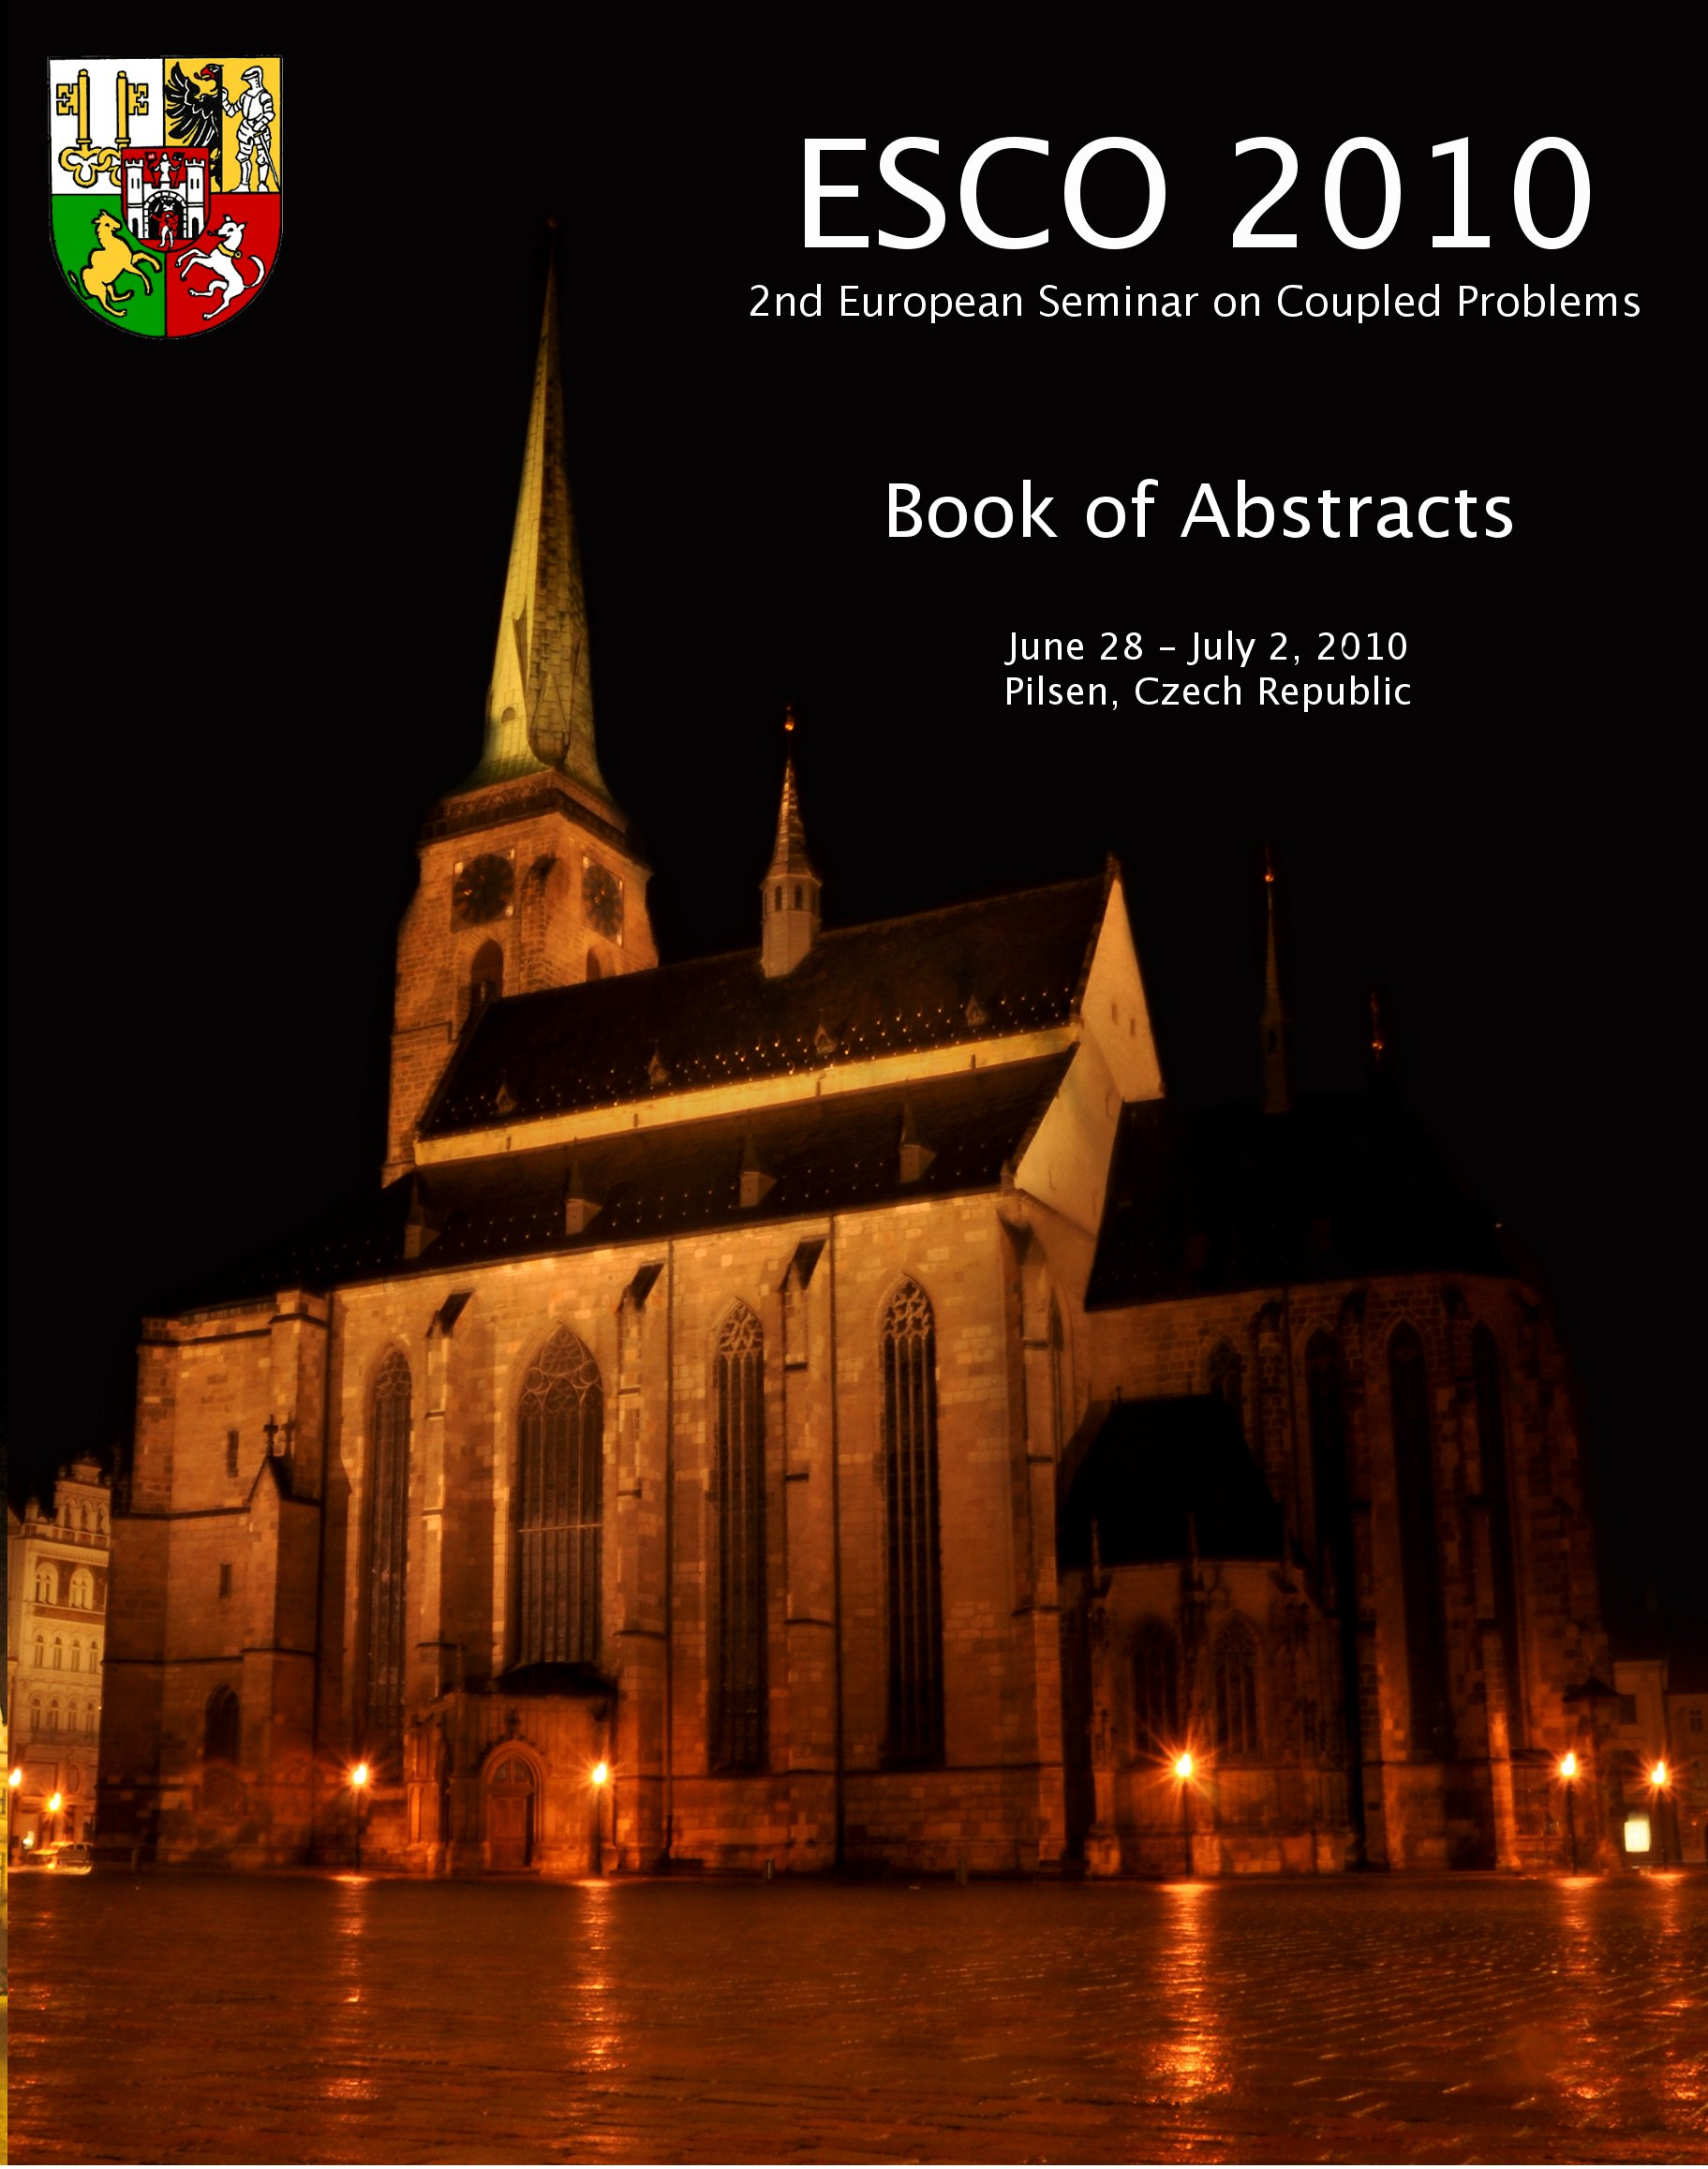
\includegraphics[width=\paperwidth,height=\paperheight]{background_plzen.jpg}%
\vfill
}}}

% BEGIN DOCUMENT
\begin{document}

% inputting background image
\AddToShipoutPicture{\BackgroundPic}

\vbox{}
\pagestyle{empty}

\newpage

\textwidth=15.5cm

\ClearShipoutPicture

\newpage

\section*{}%

\vspace*{60mm}
ISBN ???-??-????-???-?\\ \\
This is a joint publication of the 
University of Nevada (Reno), 
Desert Research Institute (Reno),
Idaho National Laboratory (Idaho Falls),
U.S. Army R\&D Center (Vicksburg), 
Institute of Thermomechanics (Prague, Czech Republic), 
and University of West Bohemia (Pilsen, Czech Republic).\\

\noindent
FEMTEC 2011:
3rd International Conference on Computational Methods in Engineering and Science\\

\noindent
\begin{tabular}{ll}
Editors: & Pavel Solin (University of Nevada, Reno \& Institute of Thermomechanics, Prague) \\
 & Glen Hansen (Idaho National Laboratory)\\
 & Pavel Karban (University of West Bohemia, Pilsen) \\
 & Chris Kees (U.S. Army R\&D Center, Vicksburg, Mississippi) \\
 & Darko Koracin, Matt Reeves (Desert Research Institute, Reno) \\
Publisher: & University of Nevada, Reno \\
 & 1664 North Virginia Street \\
 & Reno, NV 89557 - 0084\\
 & U.S.A.\\
Printed by: & XXXXXXXXX \\
 & XXXXXXXXX\\
 & XXXXXXXXX\\
Year: & 2011\\
\end{tabular}

\subsection*{Contact Information}

Mailing address:\\
FEMTEC 2011 Conference\\
Department of Mathematics and Statistics\\
University of Nevada, Reno, NV 89557 - 0084\\ 

\noindent
E-mail: {\tt femtec2011@unr.edu}\\
Web page: {\tt http://hpfem.org/events/femtec-2011/}\\
Phone: 1-775-848-7892

\chapter*{\huge FEMTEC 2011}
\vspace{-5mm}
\normalsize   
\begin{center}
3rd International Conference on Computational Methods in Engineering and Science\\
Harvey's Casino and Resort\\ 
May 9 - 13, 2011\\
\end{center}
\vspace{-3mm}

\section*{Conference topics}%

\begin{itemize}
  \item Computational methods in geosciences including, but not limited to, 
        atmospheric sciences (weather and climate), hydrology, geology, 
        atmospheric chemistry, air pollution, and related disciplines. 
  \item Computational methods in nuclear, mechanical, civil, electrical, and 
        other engineering fields. 
  \item Mesh generation and scientific visualization. 
  \item Open-source scientific computing software.
  \item Interactive browser tools, web-based computing and visualization.
  \item Python in open source scientific computing projects.
  \item Novel scientific computing tools such as SciPy, NumPy, SymPy etc.
  \item Common platforms for scientific computing, interfacing and interoperability.
\end{itemize}

\subsection*{Scientific Committee}%

%\hspace{4mm} 

\begin{itemize}
\item Valmor de Almeida (Oak Ridge National Laboratory, Oak Ridge, USA)
\item Ivo Dolezel (Czech Technical University, Prague, Czech Republic)
\item Glen Hansen (Idaho National Lab, Idaho Falls, USA)
\item Pavel Karban (University of West Bohemia, Pilsen, Czech Republic)
\item Christopher Kees (U.S. Army Engineer Research and Development Center, USA)
\item Matthew Knepley (University of Chicago, USA)
\item Darko Koracin (Desert Research Institute, Reno, USA)
\item Dmitri Kuzmin (University of Erlangen, Germany)
\item Stephane Lanteri (INRIA, France)
\item Matthias Moeller (Technical University of Dortmund, Germany)
\item Sascha Schnepp (Technical University of Darmstadt, Germany)
\item Stefan Turek (Technical University of Dortmund, Germany)
\item Gael Varoquaux (CEA Saclay, France)
\end{itemize}

\subsection*{Organizing Committee}

\begin{itemize}
\item Pavel Solin (University of Nevada, Reno and Institute of Thermomechanics, Prague)
\item Glen Hansen Idaho National Laboratory, Idaho Falls
\item Pavel Karban  (University of West Bohemia, Pilsen)
\item Christopher Kees U.S. Army Engineer R\& Center, Vicksburg
\item Darko Koracin, Matt Reeves, Desert Research Institute, Reno
\end{itemize}

\newpage
{\ }

\tableofcontents



%%%%%%%%%%%%%%%%%%%%%%%%%%%%%%%%%%%%%%%%%%%%%%%%%%%%%%%%%%%%%%%%%%%%%%%%%%%%%%%%%%%%%%%%%%%%%%%%%%%%%%%%%%%%%%%%%%%%%%%%%%%%%%%%%%%%%%%%%%%%%%%%%%%%%%%%%
\part{Abstracts of Keynote Lectures}

\pagestyle{plain}

\input dawson.tex \newpage
\input heroux.tex \newpage
\input shadid.tex \newpage


%--------------------------------------------------------------------------------------
\part{Abstracts of Contributed Lectures}

% \input bala.tex \newpage % THIS PERSON SUBMITTED A BADLY FORMATTED WORD DOCUMENT
\input berzins.tex \newpage
\input bottcher.tex \newpage
\input hakula.tex \newpage
\input hansen.tex \newpage
\input hernandez.tex \newpage
\input husanu.tex \newpage
\input jiang.tex \newpage
\input kees.tex \newpage
\input korous.tex \newpage
\input kucerova.tex \newpage
\input li.tex \newpage
\input mcalpine.tex \newpage
\input meeker.tex \newpage
\input novak.tex \newpage
\input paoluzzi.tex \newpage 
\input persson.tex \newpage
\input piskin.tex \newpage
\input sinha.tex \newpage
\input soto.tex \newpage
%\input svacek.tex \newpage    #neprijede
\input xudong_II.tex \newpage





%--------------------------------------------------------------------------------------
\newpage


\part{List of Participants}

\input addresses.tex

%--------------------------------------------------------------------------------------
%--------------------------------------------------------------------------------------
%--------------------------------------------------------------------------------------


\end{document}
